%!TEX root = ../thesis.tex

\chapter{Introduction to Fully Homomorphic Encryption}
\label{chap:fhe}


\section{Motivation}

Cryptography has experienced a tremendous boom over the past decades. In particular, Internet traffic, which used to be transmitted in plaintext, was secured by the introduction of the HTTPS protocol, which encrypts and authenticates communications between client and server.

However, one use case remains where cryptography is still ineffective, and where data is still poorly protected: delegated computation. This (vague) term encompasses all scenarios where a user sends data to a server not merely to transmit it across the Internet, but to have it processed and to receive a result in return. One can think, for example, of applications like Google Maps, where the user sends their current location and destination to a server, which then computes a route and sends it back to the user’s phone. Another example is the new generative Artificial Intelligence applications, where the user’s input is processed by an algorithm to generate text, music, or images. Finally, this also applies to cases where companies rent external servers to perform heavy computations or to host services.

The problem is that performing computations on encrypted data is a massive technological challenge, long thought to be impossible. As a result, the server must necessarily decrypt the data before processing it, which leaves the data vulnerable to any potential compromise of the server by a cyberattack.


Homomorphic encryption (Fully Homomorphic Encryption, or FHE) is the branch of cryptography that tackles this issue. Its goal is to develop encryption algorithms that allow a server to perform computations directly on encrypted data, without the need to decrypt it first. This way, an attacker has no incentive to breach the server, as all valuable data it contains remains encrypted and therefore useless. Additionally, the service provider itself does not have access to the data, ensuring full confidentiality for the user.



Figure \ref{fig:classical_usage_fhe} demonstrates a procedure of private outsourcing of computation using homomorphic encryption. We consider a use-case where a client owns some sensitive data, while a server provides some AI-based service (represented by a neural network).

\begin{enumerate}
	\item The client generates a \textit{secret key} and an \textit{evaluation key}. The former allows them to encrypt and decrypt their data, while the latter allows only to perform homomorphic computations on encrypted data, but not to acquire any information on what is actually encrypted.
	\item Using the secret key, the client encrypts its sensitive data.
	\item The client uploads the encrypted data on the server, as well as the evaluation key. Note that this evaluation key could have been sent beforehand during some user enrollment procedure.
	\item The server runs a \textit{homomorphized} version of its neural network. Using the evaluation key, it can runs the computation directly on the encrypted data to get the result the client wished. Because of the encryption layer, the server cannot gain any information on neither the input data nor the result of the computation.
	\item The server then sends back the encrypted result to the client.
	\item Using the secret key, the client can decrypt the result.
\end{enumerate}


\begin{figure}
	\centering
	%!TEX root = ../../thesis.tex
\begin{tikzpicture}
	
	%%%% Client Side (with its keys)%%%%%%%%%
	
	%%%Header%%%%%%%%%%%%%
	\node (client) at (0,0) {
		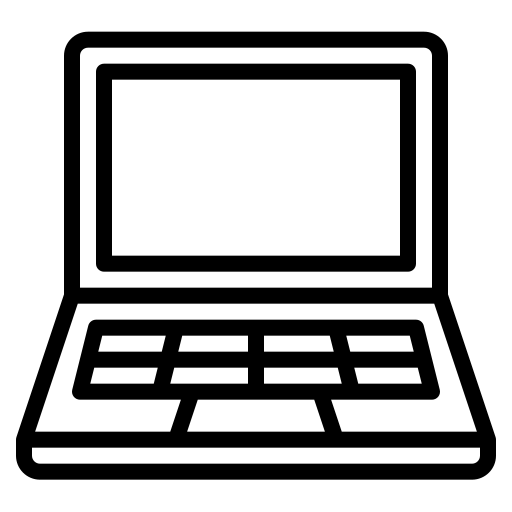
\includegraphics[width=\sizenode cm]{img/blocks_from_slides/assets/laptop.png} % Replace with your image file
	};
	\node at ($(client) + (0, 1)$) {Client};
	
	%%%%%%%%%%%%%%%%%%%%%%%
	
	%%%%%%%%% KeyGen%%%%%%%%%%%%
	
	\keygenfhe{$(client) + (1, -2)$}
	
	\node (encryption_key) at ($(keygen.west) + (-2, 0.5)$) {
		
\includegraphics[width=\sizenode cm]{img/blocks_from_slides/assets/green_key.png}
	};
	
	\node[below=0.05 of encryption_key] (evaluation_key) {
		
\includegraphics[width=\sizenode cm]{img/blocks_from_slides/assets/evaluation_key.png}
	};
	
	\draw[-latex] (keygen) -- (encryption_key);
	\draw[-latex] (keygen) -- (evaluation_key);
	
	\node (one) at ($(keygen) - (4, 0)$) {1.};
	%%%%%%%%% Chiffrement homomorphe%%%%%%%%%%%%
	
	\encfhe{$(keygen) + (-1, -3)$}
	\node (plain_data) at ($(enc_fhe.west) + (-1, 0)$) { 
		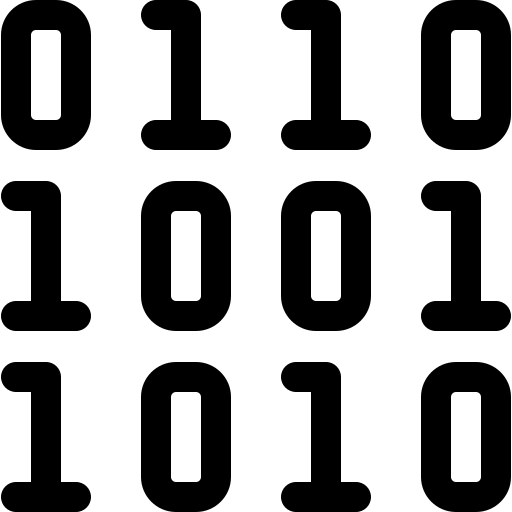
\includegraphics[width=\sizenode cm]{img/blocks_from_slides/assets/data.png} % Replace with your image file
	};
	
	\fhedata{$(enc_fhe.east) + (1, 0)$}
	
	\draw[-latex] (plain_data) -- (enc_fhe); 
	\draw[-latex] (enc_fhe) -- (data_fhe);
	
	\node (two) at ($(plain_data) - (1, 0)$) {2.};
	
	
	%%%%%Server Side %%%%%%%
	
	\node (server) at (8,0) {
		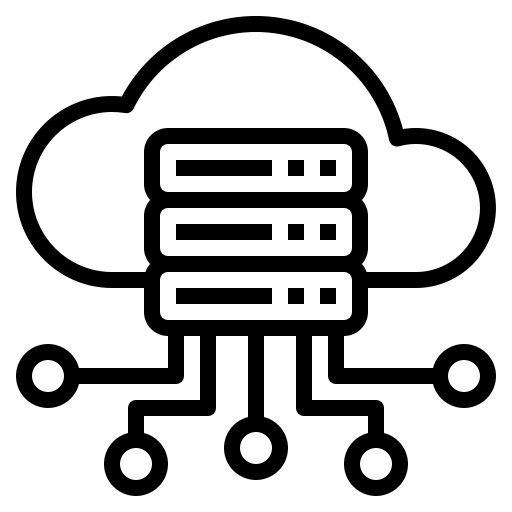
\includegraphics[width=\sizenode cm]{img/blocks_from_slides/assets/server.png} % 
	};
	
	\node at ($(server) + (0, 1)$) {Server};
	
	
%	%%%%%%%%%%Transfert de la donnée chiffrée et de la clé
%	
%	
	\fhedata{$ (4, -8) - (1, 0)$}
	\node (evaluation_key) at ($(data_fhe.east) +(1, 0)$) {
		
\includegraphics[width=\sizenode cm]{img/blocks_from_slides/assets/evaluation_key.png}
	};

	
	\draw[color=gray, thick, opacity=0.6, dash pattern=on 6pt off 3pt] ($(data_fhe) - (1, - 1)$) rectangle ++(3.5,-2);
	
	\draw[->, gray, >=stealth, line width=1mm, opacity=0.6] ($(data_fhe) - (1.5, 1.5)$) -- ++(5,0);
	
	\node (three) at ($(data_fhe) - (1.5, 0)$) {3.};
%	
      
%	%%%%%%%%%% evaluation du réseau de neurone homomorphe
%	
	\fheneuralnetwork{$(server) + (0, -11)$}
	
	\fhedata{$(fhe_neural_network.west) - (1, 0)$}
	
	\fheresult{$(fhe_neural_network.east) + (1, 0)$}
	% 
	\draw[-latex] (data_fhe) -- (fhe_neural_network); 
	\draw[-latex] (fhe_neural_network) -- (result_fhe);
	%        
	\node (four) at ($(data_fhe) - (1, 0)$) {4.};
	
	%	%%%%%%%%%%Transfert reotur%	
	%	
	\fheresult{$(4, -13)$}
	
	\draw[color=gray, thick, opacity=0.6, dash pattern=on 6pt off 3pt] ($(result_fhe) - (1, - 1)$) rectangle ++(2,-2);
%	
	\draw[<-, gray, >=stealth, line width=1mm, opacity=0.6] ($(result_fhe) - (1.5, 1.5)$) -- ++(3,0);
	
	\node (five) at ($(result_fhe) - (1.5, 0)$) {5.};
	%

	%%%%%%%%% Déchiffrement homomorphe%%%%%%%%%%%%
	
	
	\decfhe{$(enc_fhe) + (0, -11)$}
	\node (plain_result) at ($(dec_fhe.east) + (1, 0)$) { 
		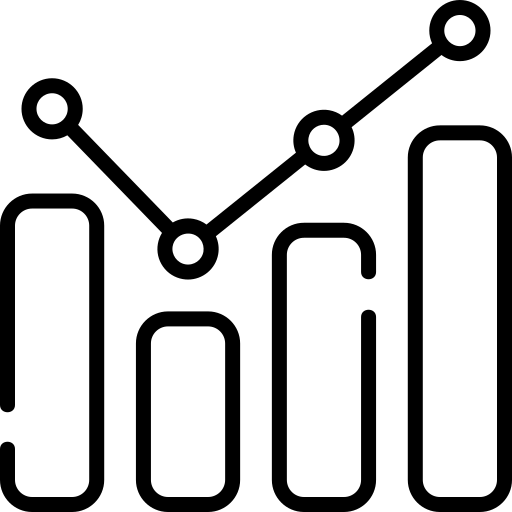
\includegraphics[width=\sizenode cm]{img/blocks_from_slides/assets/results.png} % Replace with your image file
	};
%	
	\fheresult{$(dec_fhe.west) - (1, 0)$}
%	
	\draw[-latex] (result_fhe) -- (dec_fhe); 
	\draw[-latex] (dec_fhe) -- (plain_result);
%	
	\node (six) at ($(result_fhe) - (1, 0)$) {6.};
	

	%%%%%%%%%Sep%%%%%%%
	\draw (4, 0) -- (4, -17);
	
\end{tikzpicture}


	\caption{An illustration of a protocol of outsourced computation using FHE. Hatching denotes that the homomorphized version is run.}
	\label{fig:classical_usage_fhe}
\end{figure}


\paragraph{Historical Background}

The initial appearance of the notion of homomorphic encryption in the scientific literature can be traced back to 1978, in a paper by Rivest, Adleman and Dertouzos \cite{RAD78}. They theorize the existence of \textit{privacy homomorphism}, which are \textit{encryption functions which permit encrypted data to be operated on without preliminary decryption}.

Over the following decades, research focused primarily on the development of partially homomorphic schemes, which support only a single homomorphic operation, typically either addition or multiplication. Additive homomorphisms were particularly favored in applications like electronic voting. One of the most well-known examples is the Paillier cryptosystem \cite{EC:Paillier99}.

In parallel, a different class of schemes emerged: leveled (or somewhat) homomorphic encryption schemes. These allow for both addition and multiplication, but only a limited number of operations can be performed sequentially. Notable examples include the DGHV scheme \cite{EC:DGHV10} and the original BGV scheme \cite{bgv}\footnote{Although these schemes were actually shown to be bootstrappable (see Section \ref{sec:gentry_bootstrapping}), the bootstrapping process was too inefficient to be practical.}.

Interestingly, the bounded depth of computation in these schemes arises from distinct causes. In DGHV, the size of the integers in the ciphertexts grows with each operation, eventually becoming computationally prohibitive. In BGV, it is the noise introduced during encryption that increases until it overwhelms the signal, rendering the ciphertext undecipherable. In both cases, a critical resource (either magnitude or noise) accumulates irreversibly, ultimately preventing further computation.

This bound was suddenly removed in 2009 in a groundbreaking construction by Gentry, wich opened the door to a very fast development of the field in the following years. We present this transformative result in the next section.

\section{The Bootstrapping : Breakthrough Construction}
\label{sec:gentry_bootstrapping}


In 2009, Craig Gentry publishes the breakthrough paper \textit{Fully Homomorphic Encryption using Ideal Lattices} \cite{STOC:Gentry09}. In this work, he introduces the first ever fully homomorphic encryption scheme. Its main idea is the \textit{bootstrappability} of a scheme.

Bootstrappability is the ability of a scheme to evaluate homomorphically its own decryption circuit. Gentry shows that if a scheme achieves bootstrappability, then it achieves fully homomorphic encryption. Building on this theoretical result, he constructs a lattice-based bootstrappable scheme and demonstrates the first ever example of fully homomorphic scheme. Since this foundational work, lattice-based constructions have remained the only serious candidate for fully homomorphic encryption. 

Such homomorphic schemes work by injecting some small random noise in the plaintext data before encryption. Its role is to ensure security, relying on computational hardness assumptions such as Learning With Errors ($\LWE$) (we explain it further in Section \ref{sec:hardness_assumptions}). Because the noise is small, it can be easily removed during decryption by a simple rounding operation. 

Gentry's original scheme offered homomorphic additions and multiplications. However, because the plaintext messages are noisy, these operations increase the noise in the ciphertexts. So, if too many operations are performed, the noise gets so large that it becomes preponderant and blows the meaningful information contained in the ciphertexts.

This is where bootstrappability comes in. It gives access to an operation (the \textit{bootstrapping}) that decrypts homomorphically the noisy ciphertexts. But how can this help to achieve FHE ?

Imagine the server has a ciphertext $\vec c_1$ encrypting the (noisy) message $m +e_1$ under the secret key $\vec s_1$, where $m$ is the plain message and $e_1$ denotes the noise. Let us say that $\vec c_1$ is the output of a circuit of homomorphic operations, so the noise $e_1$ is rather large. If we want to keep computing without losing information, we need to reduce the noise by a bootstrapping. 

To do so, the client needs to give to the server a \textit{bootstrapping key} $\BSK$. In order to create it, the client can treat the secret key $\vec s_1$ as a message and encrypt it under another secret key $s_2$ to produce $\BSK = \texttt{Enc}_{s_2}(s_1)$. Now, if the server computes \textit{homomorphically} the decryption of $c_1$ using $\BSK$, it retrieves an encryption $\vec c_2$ of the same message under the secret key $\vec s_2$. But because, decryption removes noise, $e_1$ disappears and the ciphertext is fresh again!

Actually, \textit{all} the noise does not get removed (this would not be desirable, because all the security of the encryption relies on the presence of noise in the ciphertexts). As there is some noise in $\BSK$, the result $\vec c_2$ carries some noise $e_2$. But if things are well dimensioned, it is possible to get $e_2 \ll e_1$ and so retrieve some room for further computations. We illustrate the bootstrapping principle in Figure \ref{fig:bootstrapping_principle}.


Gentry's original scheme was merely theoretical, because the homomorphic operations and in particular the bootstrapping was extremely slow. But since then, significant improvements have been achieved in FHE efficiency. Modern schemes are on the verge of being usable in practice for some use-cases. In the next section, we give a tour of the modern schemes and libraries that makes the FHE landcape as of today.



\begin{figure}
	\centering
	%!TEX root = ../../thesis.tex
\begin{tikzpicture}
	\bootstrapping{$(0, 0)$}
	
	\fhedatabis{$(bootstrapping.east) + (2, 0)$}
	
	\fhedata{$(bootstrapping.west) - (2, 0)$}

	\bootstrappingkey{$(bootstrapping.south) - (0, 2)$}
	
	\draw[-latex] (data_fhe) -- (bootstrapping); 
	\draw[-latex] (bootstrapping) -- (data_fhe_bis);
	\draw[-latex] (bootstrapping_key) -- (bootstrapping);
	
	\node at ($(data_fhe) - (1, -1)$){\verticalgauge{90}};
	
	\node at ($(bootstrapping_key) - (1, 1)$){\verticalgauge{20}};
	
	\node at ($(data_fhe_bis) - (1, -1)$){\verticalgauge{40}};
\end{tikzpicture}


% #1 = scale, #2 = height, #3 = level (0–100)

	\caption{High-level overview of the bootstrapping principle. Hatching denotes the fact that the operation is ran homomorphically. The gauges denotes indicative noise levels for the ciphertexts.}
	\label{fig:bootstrapping_principle}
\end{figure}


\section{Current Landscape of the FHE Schemes and Libraries}
\label{sec:landscape}

After a decade of research, homomorphic schemes have evolved to stabilize around two main paradigms. We present both by their main representatives: TFHE \cite{JC:CGGI20} and CKKS \cite{AC:CKKS17}. They have quite different (and complementary) philosophies of computing, and lead to radically different design choices when used:


\paragraph{TFHE:} This scheme relies on a very low-latency\footnote{by FHE standards} bootstrapping operation. It manipulates small limbs of data of a few bits, and operates \textit{exact} computations on them.


\paragraph{CKKS:} CKKS has quite opposite features than TFHE. It relies on a \textit{approximate} paradigm fo the computations, so is quite appropriate for floating-point computations. Moreover, it supports SIMD (Same Instruction Multiple Data) within its ciphertexts, so it allows for heavy parallelization. While its bootstrapping is quite heavy and appeared later in the literature \cite{EC:CHKKS18}, a lot of advancements happened in the last few years making it closer to practical \cite{EC:CheChiSon19, RSA:HanKi20, AC:KPKKM22}.


We should also mention BFV/BGV \cite{C:Brakerski12, bgv, EPRINT:FanVer12}, that share most of the properties of CKKS. However these constructions do not work with approximate floating-point computation, but rather with exact computations over large integer rings.


Several libraries implement these schemes, facilitating their adoption. For TFHE, we can mention tfhe-rs \cite{tfhe-rs}  and TFHEpp \cite{TFHEpp}. For CKKS, we can mention HEAAN \cite{heaan} and Lattigo \cite{lattigo}. Finally, OpenFHE \cite{OpenFHE} is an attempt at constructing a universal library that supports all the schemes and allows conversions.


These libraries target users familiar with FHE, and offer quite low-level API. One of the issue slowing down the massive adoption of FHE is the difficulty of developing concrete applications from the cryptographic primitives. A layer of compilation is thus required from ``plaintext'' programming to homomorphic code. Such projects of homomorphic compiler include Concrete \cite{Concrete} and heir \cite{HEIR}.


Another active line of research is hardware acceleration. Quite promising theoretical results have been achieved \cite{TCHES:GVPHMS23, EPRINT:BBTV23a, EPRINT:CPBFSJ23, EPRINT:KHMR24} and the first ``FHE-tailored'' chips have started to be produced. Such hardware include NTT/FFT-dedicated accelerators, as these operations account for the largest part of the computations. 


Some standardization projects are arising \cite{HomomorphicEncryptionSecurityStandard, call_nist}, which would be an important step for the adoption of FHE in practice.
 	


\section{Security Properties}


In cryptography, the security of a scheme is modelized by a \textit{security game}. In an idealized world, a challenger running the scheme is opposed to a polynomial-time attacker. This attacker has access to \textit{oracles} that they can query. For encryption scheme, one of these games is the \textit{indisguishability game}: the attacker picks two messages and sends them to the challenger. The challenger flips a coin and encrypts one of the messages at random. They send this ciphertext (named the \textit{challenge ciphertext}) to the attacker, who has to guess which message has been encrypted. If the attacker can do better that random guessing (so guess right with probability larger than 0.5), we say that they have a \textit{non-negligible advantage}, indicating a vulnerability against the type of attack.

Usually, the ``graal'' for encryption schemes is \textsf{CCA2} security (or \textit{adaptative chosen-ciphertext security}). In the corresponding game, the attacker has access to an encryption and a decryption oracle, that they can query both before and after having received the challenge ciphertext, with the exception that they are forbid to query the decryption oracle directly on the challenge ciphertext.



By design, homomorphic schemes cannot achieve such security property because they are intrinsically \textit{malleable}. So a trivial attack would be to homomorphically add an encryption of zero to the challenge ciphertext and query the decryption oracle on the result. The oracle would accept the decryption and output the message, completely breaking the security of the scheme.

Actually, things are even worse: if the scheme is bootstrappable, then even \textsf{CCA1} security is unachievable. This corresponds to a \textit{non-adaptative chosen-ciphertext security}, the difference with \textsf{CCA2} being that the attacker is no longer allowed to query the decryption oracle after having seen the challenge ciphertext (so it modelizes a weaker security property). To understand the attack, recall that in Gentry's blueprint, the bootstrapping key is an encryption of the secret key. So, by querying the decryption oracle with the bootstrapping key, the attacker may recover the secret key and decrypt any ciphertext sent by the challenger. Some attacks are even possible with more constrained decryption oracles: for example \cite{SAC:LMSV11} demonstrates attacks with only an access to an oracle that tells if a ciphertext is valid or not, which seems a very practical concern.


Because these advanced security properties are so hard to achieve, the \textit{de facto} standard for FHE schemes has become \textsf{CPA} security (where the attacker has only access to an encryption oracle and no decryption oracle). This is the level of security targeted by most applied libraries. However, such security level is not sufficient in practice for most of the use-cases of FHE.


The problem has first been revealed in the work of \cite{EC:LiMic21} for approximate homomorphic schemes. In their work, they leverage the fact that the decryption function leaks the noise in ciphertexts to mount a secret-key recovery attack. They named this framework $\textsf{CPA}^\textsf{D}$ ($\cdot ^ \textsf{D}$ denoting the use of the output of the Decryption algorithm). To be protected against such attacks, users should be prohibited to disclose the results of decrypted messages. But in some use-cases (such as Multi-Party Computations), it is necessary to share the decrypted message with other users. So the outputs of the decryption algorithm should be protected by injecting random noise to flood the leaked information \cite{EPRINT:CheHonKim20}. Actually, further works \cite{C:CSBB24, CCS:CCPSS24} have shown that non-approximate schemes are also vulnerable to $\textsf{CPA}^\textsf{D}$ attacks: instead of exploiting the noise leakage, the attacker can actively tamper with the noise in ciphertexts to trigger decryption errors and harvest information to mount a key-recovery attack.


What these attacks show is that FHE by itself is not sufficient to build secure applications in the real world. To prevent against tampering of ciphertexts, \textsf{CPA} secure FHE schemes needs to be augmented with some machinery to prove the well-formedness of ciphertexts. Some literature on the topic has developed in the recent years, notably the works of \cite{EC:ManNgu24, CiC:BCFPPR25}. They develop a new security notion of \textsf{vCCA} (for \textit{verified chosen ciphertext security}) and implement it in practice with SNARKS \cite{SNARKS} (succing non-interactive argument of knowledge). 


